\section{关系}
\subsection{二元关系}
一个从集合$A$到集合$B$的二元关系是有序对的集合$R$,其中每个有序对的第一个元素取自$A$,第二个元素取自$B$。

使用$aRb$表示$(a,b) \in R$,称$a$与$b$有关系$R$.

集合$A$的关系是从$A$到$A$的关系。

例如:$A = \{ 1,2,3,4,5 \}$,$A$上的关系$R=\{ (a,b) \mid a \text{整除} b \}$中有哪些有序对?

\subsubsection*{二元关系的性质}
\begin{itemize}
    \item 一个从集合$A$到集合$B$的二元关系是$A \times B$的子集。
    
    \item 若对于每个元素$a \in A$有$(a,a) \in R$,则称集合$A$上的关系$R$是自反的。
    
    \item 对于元素$a,b \in A$,若只要$(a, b) \in R$就有$(b,a) \in R$,则称集合A上的关系$R$是对称的。

    对于元素$a,b \in A$,仅当$a = b$时,有$(a,b) \in R$和$(b,a) \in R$,则称集合A上的关系$R$是反对称的。

    \item 对于元素$a,b,c \in A$,若$(a, b) \in R$且$(b,c) \in R$,则$(a,c) \in R$,则称集合A上的关系$R$是传递的。

    \item 设$R$是从集合$A$到集合$B$的关系,$S$是从集合$B$到集合$C$的关系,$R$和$S$的合成是由有序对$(a,c)$构成的关系,其中$a \in A, c \in C$,并且对于它们存在一个元素$b \in B$使得$(a,b) \in R, (b,c) \in S$。用$S \circ R$表示$R$和$S$的合成。

    \item 设$R$是集合$A$上的关系,则幂$R^n$递归地定义为$R^1 = R, R^{n+1} = R^n \cdot R$.

    当且仅当对于$n=1,2,3$有$R^n \subset R$时,集合$A$上的关系$R$是传递的。
\end{itemize}

\subsubsection*{二元关系的表示}
二元关系的表示可以使用矩阵、有向图。

使用矩阵表示二元关系,矩阵中的元素的位置代表了集合中的不同的元素,矩阵中的元素的值为1或0,表示该元素对应的集合中的两个元素之间有无关系。

使用有向图表示二元关系,每个节点代表集合中的一个元素,节点之间的有向线段表示元素之间的关系,如有从节点$a$指向节点$b$的线段,则表示存在关系$(a,b)$.

\subsection{$n$元关系}
在集合$A_1, A_2, \cdots, A_n$上的$n$元关系是$A_1 \times A_2 \times \cdots \times A_n$的子集。其中$A_1, A_2, \cdots, A_n$称为关系的域,$n$叫做关系的阶。

例如,关系数据类型中的每个字段都是一个$n$元组,一条记录就是就是一个$n$元关系。

以下是$n$元关系的一些运算:
\begin{itemize}
    \item \uline{选择运算}:设$R$是$n$元关系,$C$是$R$中元素可能满足的条件,则选择运算$s_c$是将$R$映射到$R$中满足$C$的所有$n$元组构成的$n$元关系。也即选择满足条件的关系(记录)。

    \item \uline{投影}:投影$P_{i_1, i_2, \cdots, i_m}$是将$n$元组$a_1,a_2,\cdots,a_n$映射到$m$元组,$m \le n$. 也即将$n$元组中位置为$i_1, i_2, \cdots, i_m$的元素保留,其它删去。

    例如,数学老师只选取某个班级期末成绩单中的姓名、学号、数学成绩,而删去其它科目的成绩。

    \item \uline{连接}:设$R$是$m$元关系,$S$是$n$元关系,$p \le m, p \le n$,则连接$J_p(R,S)$是$m + n - p$元关系,包含$(a_1, a_2, \cdots, a_{m-p}, c_1, c_2, \cdots, c_p, b_1, b_2, \cdots, b_{n-p})$,其中,$m$元组$(a_1, a_2, \cdots, a_{m-p}, c_1, c_2, \cdots, c_p)$属于$R$,$n$元组$(c_1, c_2, \cdots, c_p, b_1, b_2, \cdots, b_{n-p})$属于$S$

    例如,关系$R$为由(课程,课程号)构成,关系$S$由(课程号,教室号,时间)构成。则连接$J_1(R,S)$是由(课程,课程号,教室号,时间)构成,课程号为重叠的部分。
\end{itemize}

\subsection{闭包}
设$R$是集合$A$上的关系,$R$可能具有或不具有某种性质$P$。若存在关系$S$ \fbox{包含$R$} \fbox{具有某种性质$P$},且$S$是最小的(也即$S$是所有的\fbox {包含$R$} \fbox {具有某种性质$P$} 的关系的子集),则称$S$为$R$关于$P$的闭包。

例如集合$A = \{1,2,3\}$,关系$R = \{(1,1), (2,1), (3,2)\}$不是自反的,我们增加两个元素$(2,2), (3,3)$,构建关系$S$为自反的,称$S$是$R$的自反闭包。还有传递闭包、对称闭包。

\subsubsection*{传递闭包}
设$R$是集合$A$上的关系,连通性关系$R^*$由对$(a,b)$构成,使得在$R$的有向图中存在一条长度至少为1的路径。也即,在关系$R$中不管中间经过多少元素,只要能从元素$a$传递到元素$b$,则对$(a,b)$就会出现在$R^*$中。

\begin{itemize}
    \item 设$R$是集合$A$上的关系。集合$A$的有向图中,$a,b$之间存在长度为$n$的路径,等价于$(a,b) \in R^n$。因此,连通性关系$R^* = \displaystyle \bigcup _{i=1}^n R^i$.
    \item 关系$R$的传递闭包等于连通性关系$R^*$.
    \item 设$R$是集合$A$上的关系,集合$A$有$n$个元素,若存在一条从$a$到$b$的长度至少为1的路径,则存在一条长度不超过$n$的这种路径。若$a \neq b$,则则存在一条长度不超过$n-1$的这种路径。
    \item 设$\bf M_R$是$n$元素集合上的关系$R$的0-1矩阵,则传递闭包$R^*$的0-1矩阵为
    \[\bf M_{R^*} = \bf M_R \vee \bf M_{R^2} \vee \cdots \vee \bf M_{R^n}\]
\end{itemize}

\subsubsection*{沃舍尔算法}
沃舍尔算法用来计算传递闭包,也称为罗伊-沃舍尔算法。

理解沃舍尔算法需要以下概念:
\begin{itemize}
    \item 设$v_i$为集合的元素,$v_1,v_2,\cdots,v_n$为$n$个元素的任意排列。
    \item \uline{内点}:设路径$a, x_1, x_2, \cdots, x_k, b$,其中$x_1, x_2, \cdots, x_k$为$k$个内点。
\end{itemize}

设$R$为$n$元素集合上的关系,取集合中所有元素的一个排列,记为$v_1,v_2,\cdots, v_n$.沃舍尔算法需要构建一系列$n$阶0-1矩阵:$\bf W_0, \bf W_1, \cdots, \bf W_n$,其中,$\bf{W_k}$$= [w _{ij}^{[k]}]$.当元素$v_i$到元素$v_j$之间存在一条路径,且该路径经过的所有内点为前$k$个元素$v_1, v_2, \cdots v_k$的子集时,$w _{ij}^{[k]} = 1$,否则,$w _{ij}^{[k]} = 0$.

当$k=0$时,从$v_i$到$v_j$之间没有内点,因此$\bf W_0 = M_R$;当$k=n$时,从$v_i$到$v_j$之间的内点可以是集合中除起点终点外的任意元素,因此$\bf W_n = M_{R^*}$。

在已知$W_{k-1}$时,从$v_i$到$v_j$有两种情况:(1)$w _{ij}^{[k-1]}=1$(2)$w _{ij}^{[k-1]}=0$.要求$W_k$,需要在可选内点的序列$v_1, v_2, \cdots, v_{k-1}$中增加点$v_k$.
    \begin{enumerate}
        \item 若$w _{ij}^{[k-1]} = 1$,则$w _{ij}^{[k]}=1$.即已经有路径存在。
        \item 若$w _{ij}^{[k-1]} = 0$,此时若$w _{ik}^{[k-1]} = w _{kj}^{[k-1]} = 1$,即增加的点$v_k$使得可以从$v_i$传递到$v_k$,再从$v_k$传递到$v_j$,实现从$v_i$传递到$v_j$,则$w _{ij}^{[k]} = 1$.
    \end{enumerate}
综上所述,可得
\[ \omega _{ij}^{[k]} = \omega _{ij}^{[k-1]} \vee (\omega _{ik}^{[k-1]} \wedge \omega _{kj}^{[k-1]}) \]

由于已知$\bf W_0$,依次计算$\bf W_1, \bf W_2, \cdots, \bf W_n$,即可得到传递闭包$R^*$的0-1矩阵$\bf M_{R^*} = \bf W_n$.

\subsection{等价关系}
如果集合$A$上的关系是自反的、对称的和传递的,则这个关系称为等价关系。

如果集合中的两个元素$a,b$因为等价关系而相联系,则称他们是等价的。

设$R$是集合$A$上的等价关系,与集合$A$上的元素$a$有关系的所有元素的集合叫做$a$的等价类。记作$[a]_R$.换句话说,$[a]_R = \{s \mid (a,s) \in R\}$.(如果命题中只讨论一个关系,如只考虑关系$R$,等价类的下标可以省略。)

\begin{itemize}
    \item 设$R$是集合$A$上的等价关系,则以下命题等价:(1)$aRb$ \quad (2)$[a] = [b]$ \quad (3)$[a] \cap [b] \neq \emptyset$.

    简单的证明:
    \begin{enumerate}
        \item (1) $\rightarrow$ (2):当$(a,b) \in R$,假设存在一个元素$c \in A$使得$(a,c) \in R$(此元素可能为$a$自身),由对称性$(c,a) \in R$,则由传递性 $(c,b) \in R$,可证,凡是属于$[a]$的元素皆属于$[b]$,也即$[a] \subset [b]$。同理可证$[b] \subset [a]$,因此$[a] = [b]$.

        \item (2) $\rightarrow$ (3):当$[a] = [b]$时,由于$R$的自反性,\uline{等价类必不为空},故存在元素假设记为$c \in [a], c \in [b]$,故$[a] \cap [b] \neq \emptyset$.

        \item (3) $\rightarrow$ (1):当$[a] \cap [b] \neq \emptyset$,即存在元素假设记为$c \in [a], c \in [b]$,也即$(a,c) \in R, (b,c) \in R$。由对称性和传递性,$(a,b) \in R$.
    \end{enumerate}
    通过上述证明的组合,可得上述命题是等价的。

    \item 设$R$是集合$S$上的等价关系,那么$R$的等价类构成$S$的划分。相反,若给定集合$S$的一个划分$\{A_i \mid i \in I\}$,则存在一个等价关系$R$,其等价类为$A_i(i \in I)$.

    $R$上的等价类之间有两种情况(1)$[a] \cap [b] = \emptyset$(2)$[a] \cap [b] \neq \emptyset$.当$[a] \cap [b] \neq \emptyset$时,由上述命题的等价关系$[a] = [b]$,也即,$R$上的等价类要么相同,要么没有交集。因此,$R$上的等价类将$S$中的划分成不同的部分,在同一部分中的元素的等价类相同,为该部分;不同部分之间的元素的等价类没有交集。

    当给定一个划分时,每一个子集是一个等价类,通过等价类形成等价关系。
\end{itemize}

\subsection{偏序}
如果集合$S$上的关系$R$是自反的、反对称的和传递的,则这个关系称为偏序。
$(S,R)$称为偏序集。

\begin{itemize}
    \item 偏序集$(S, \preccurlyeq)$中,如果$a \preccurlyeq b$或$b \preccurlyeq a$,则称元素$a,b$是\uline{可比的};否则,称为不可比的。
    \item 偏序集$(S, \preccurlyeq)$中,如果$S$中的每对元素都可比,则$S$称为\uline{全序集或线序集},也称为链。此时$\preccurlyeq$叫做全序或线序。
    \item 偏序集$(S, \preccurlyeq)$中,如果$\preccurlyeq$全序,且$S$中的每个非空子集都有最小元素,称它为\uline{良序集}。
\end{itemize}
\uline{良序归纳定理}:设集合$S$是一个良序集。如果对于所有的$y \in S$,当对于所有的$x \in S, x \prec y$,$P(x)$均成立时,$P(y)$成立,则对于所有的$x \in S$,$P(x)$恒成立。\\

其它的一些概念:
\begin{itemize}
    \item \uline{字典顺序}:两个序列中第一个元素小的在前,如果相等,则第二个元素小的在前,以此类推。

    \item 哈塞图:一个偏序集中的集合的有向图,去除表示自反的环(元素指向自身),去除可以用更短的路径组合出的表示传递的路径,将起点放在最下、终点在最上,最后化简为一个包含足够信息的图,称为哈塞图。

    \begin{figure*}[htbp]
        \centering
        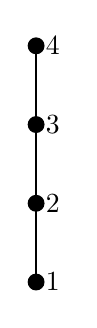
\begin{tikzpicture}
            \filldraw (0,0) circle (.1) node[right] {$1$}
                (0,1) circle (.1) node[right] {$2$}
                (0,2) circle (.1) node[right] {$3$}
                (0,3) circle (.1) node[right] {$4$};
            \draw [line width=1pt] (0,0)--(0,3);
        \end{tikzpicture}
        \caption{$(\{1,2,3,4\}, \leq)$的哈塞图}
    \end{figure*}

    \item 极大值和极小值
    \item 上界和下界:对于偏序集$(S, \preccurlyeq)$的子集$A$,若存在元素$u \in S$使得$A$中的所有元素$a_i \preccurlyeq u$,则称$u$为$A$的一个上界。下界的定义类似。
    \item 最小上界和最大下界。在子集$A$的所有上界中,如果上界$x$小于其它任何的上界,则称$x$为$A$的最小上界。同理,在子集$A$的所有下界中,如果下界$x$大于其它任何的下界,则称$x$为$A$的最大下界。分别记作$\mathrm{glb} (A)$和$\mathrm{lub} (A)$.

    \item 若一个偏序集中的每一对元素都有最小上界和最大下界,则称此偏序集为\uline{格}。
\end{itemize}

\subsubsection*{拓扑排序}
如果只要$aRb$就有$a \preccurlyeq b$,则称一个全序$\preccurlyeq$和一个偏序$R$是相容的。从一个偏序构造一个相容的全序的过程称为拓扑排序。

每个有穷非空偏序集都有极小元素。

在又穷的偏序集$(A, \preccurlyeq)$中,由上述结论,选择一个最小元素$a_1$;接下来对于偏序集$(A-\{ a_1 \}, \preccurlyeq)$,若其非空,再从中选择一个最下元素$a_2$;接下来对于偏序集$(A-\{ a_1, a_2 \}, \preccurlyeq)$,若其非空,再从中选择一个最小元素$a_3$;\ldots 因为$A$是有穷集合,此过程必能结束。得到最终序列(全序)
\[ a_1, a_2, \cdots, a_n \]

\section{图}
\subsection{图的术语与表示}
图$(V, E)$由非空顶点集$V$和边集$E$组成,分为无向图和有向图。

没有环和多重边的图为简单图。

\subsubsection*{基本概念}
在无向图中,由一条边\uline{连接}或\uline{关联}的两个顶点$u,v$称为邻接,可以记作$\{u, v\}$,$u,v$称为该边的端点。

在有向图中,由一条边连接$u,v$时,称为$u$邻接到$v$,可以记作$(u,v)$.此时,$u$为起点,$v$为终点。\\

顶点的\uline{度}:
\begin{itemize}
    \item 无向图中顶点的度指与该顶点关联的边的数目,特殊的,顶点上的环为该顶点贡献双倍的度。记作$\deg (v)$.
    \item 有向图中顶点的\uline{入度}是以该顶点为终点的边的数目,记作$\deg ^- (v)$.顶点的\uline{出度}是以改顶点为起点的边的数目,记作$\deg ^+ (v)$.
\end{itemize}

\subsubsection*{性质}
\begin{itemize}
    \item \uline{握手定理}:设$G = (V,E)$是有$n$条边的无向图,则$2n = \displaystyle \sum _{v \in V} \deg (v)$.

    \item 无向图有偶数个奇数度的顶点。

    \item 设$G = (V,E)$是有向图,则$\displaystyle \sum _{v \in V} \deg ^- (v) = \sum _{v \in V} \deg ^+ (v) = \lvert E \rvert$.
    \item 子图和并图
    
\end{itemize}

\subsubsection*{一些特殊的简单图}
\begin{itemize}
    \item 完全图$K_n$:每对不同顶点之间都恰有一条边的简单图。
    \item 圈图$C_n$:由顶点$v_1, v_2, \cdots, v_n$和边$\{v_1, v_2\}, \{v_2, v_3\}, \cdots, \{v_{n-1}, v_n\}, \{v_n, v_1\}$组成的简单图。
    \item 轮图$W_n$:轮图$W_n$是在圈图$C_n$的基础上增加一个顶点,该顶点与圈图中的所有顶点相连。(注意:$W_n$有$n+1$个顶点。)
    \item $n$立方图$Q_n$:用$2^n$个顶点表示$n$位二进制位串,当两个位串只相差一位,其对应的顶点相连。
\end{itemize}

\subsubsection*{偶图}
如果可以把简单图$G$的顶点分成两个不相交的非空集合$V_1,V_2$,使得$G$的所有边的一个端点来自$V_1$,另一个端点比来自$V_2$,满足这样条件的图$G$称为偶图。此时,称$(V_1,V_2)$为$G$的二部划分。

如果一个简单图的每个顶点可以染成两种颜色中的一种,且相邻接的顶点不被染成同一种颜色,等价于该图为一个偶图。

\subsubsection*{图的表示}
\begin{itemize}
    \item 对于简单图,可以使用邻接矩阵。需要将图的顶点排序,作为矩阵中元素的行号和列号,无向图的邻接矩阵中使用0-1值表示两个点之间是否有边,无向图的邻接矩阵是一个对称阵;有向图的邻接矩阵中使用0-1值表示从行号到列号是否有边,有向图的邻接可以是非对称阵。对于非简单图,只需将矩阵中的0-1值换成边数即可。
    \item 对于稀疏的图,可以使用邻接表,节省空间。邻接表中的表项,id为每个顶点,内容为与改顶点直接相连接的其它顶点。
    \item 无向图还可以使用关联矩阵,将图的顶点排序作为矩阵的行号,边排列作为矩阵的列号,矩阵中的元素值表示其行号对应顶点和列号对应边之间是否相关联,或者多重边时表示重数。
\end{itemize}

\subsubsection*{同构}
设$G_1 = (V_1, E_1)$和$G_2 = (V_2, E_2)$是简单图,若存在一对一的和映上的从$V_1$到$V_2$的函数$F$,且$f$对于$V_1$里所有的$a$和$b$来说,$a,b$在$G$里相邻当且仅当$f(a), f(b)$在$G_2$里相邻,就称$G_1,G_2$是同构的,这样的函数$f$称为同构。

判断两个图是否同构很难,但是判断两个图不同构相对简单。若两个图有不一样的某条性质,如不同数量的边或顶点、不同数量的相同度的边、不同数量的相同长度的回路等,则两个图不同构。

\subsection{连通性}
通路是边的序列。若通路或回路不重复第包含相同的边,则它是简单的。

\begin{itemize}
    \item 若无向图每一对不同的顶点之间都有通路,则该图称为连通的。在连通无向图的每对顶点之间都存在简单通路。
    \item 若有向图每一对不同的顶点,如$(a,b)$,有从$a$到$b$和从$b$到$a$的通路,则该图是强连通的。若在有向图的底图中,任何两个顶点之间都有通路,则该有向图是若连通的。
    \item 底图:把有向图中的每条有向边改为无向边,所得的无向图是该有向图的底图。
    \item 设$G$是带有相对于顶点顺序$v_1,v_2,\cdots,v_n$的邻接矩阵$\bf A$的图(允许带有无向或者有向边、多重边和环),从$v_i$到$v_j$的长度为$r$的不同通路的数目等于$\bf A^r$的第$(i,j)$项,其中$r$是正整数。
\end{itemize}

\subsubsection*{欧拉通路和哈密顿通路}
\begin{itemize}
    \item 欧拉回路、欧拉通路:图$G$的欧拉回路是包含$G$所有边的简单回路,图$G$的欧拉回路是包含$G$所有边的简单通路。
    
    连通多重图具有欧拉回路当且仅当它的每个顶点都有偶数度。

    连通多重图具有欧拉通路但是没有欧拉回路当且仅当它恰有2个奇数度顶点。

    \item 哈密顿通路、哈密顿回路:设图$G$里,经过所有顶点但是不重复经过同一个顶点的通路,称为哈密顿通路。在哈密顿通路的基础上,增加由终点到起点的边构成的回路,称为哈密顿回路。

    不能找到一个哈密顿回路的等价描述,但是有一些判断图有哈密顿回路的充分条件:
    \begin{itemize}
        \item 狄拉克定理:若$G$是带有$n$个顶点的连通简单图,$n \ge 3$,并且$G$中每个顶点的度都至少为$n/2$,则$G$有哈密顿回路。
        \item 奥尔定理:若$G$是带有$n$个顶点的连通简单图,$n \ge 3$,并且对于$G$中每一对不相邻的顶点$u,v$来说,都有$\deg (u) + \deg (v) \ge n$,则$G$有哈密顿回路。
    \end{itemize}
    
    国际象棋中马在$m \times n$的棋盘上的周游等价于求表示马在该棋盘上合法移动的图的哈密顿通路。
\end{itemize}

\subsubsection*{带权图的最小通路}
给每条边赋上一个数的图称为带权图。

求带权图两个顶点之间的最短通路,比如旅行商问题。有不同的算法,如迪克斯特拉算法。以下图为例:

\begin{figure*}[htbp]
    \centering
    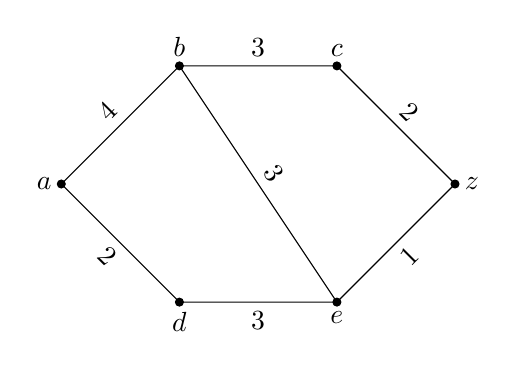
\begin{tikzpicture}
        \filldraw (0,1.5) circle (.05) node[left] {$a$}
            (1.5,3) circle (.05) node[above] {$b$}
            (3.5,3) circle (.05) node[above] {$c$}
            (1.5,0) circle (.05) node[below] {$d$}
            (3.5,0) circle (.05) node[below] {$e$}
            (5,1.5) circle (.05) node[right] {$z$};
        \draw (0,1.5)--(1.5,3) node[midway,sloped,above] {4}
            (1.5,3)--(3.5,3) node[midway,sloped,above] {3}
            (3.5,3)--(5,1.5) node[midway,sloped,above] {2}
            (0,1.5)--(1.5,0) node[midway,sloped,below] {2}
            (1.5,0)--(3.5,0) node[midway,sloped,below] {3}
            (3.5,0)--(5,1.5) node[midway,sloped,below] {1}
            (1.5,3)--(3.5,0) node[midway,sloped,above] {3};
    \end{tikzpicture}
    \caption{带权的简单图}
\end{figure*}

\begin{align*}
    & \{a, b\} > \{a, d\}, min = \{a ,d\} \\
    & \{a, b\} < \{a, d, e\}, min = \{a,b\} \\
    & \{a, b, c\} = \{a, b, e\} > \{a, d, e\}, min = \{a, d, e\}\\
    & \{a, b, c\} = \{a, b, e\} > \{a, d, e, z\}, min = \{a, d, e, z\}\\
    & \text{end.}
\end{align*}

迪克斯特拉算法求出的连通简单无向带权图里两个顶点之间的最短通路的长度。需要$O(n^2)$次运算。

\subsection{可平面的图}
若可以在平面里画出一个图且边没有任何交叉,则这个图是可平面的,这种画法称为这个图的平面表示。

\begin{itemize}
    \item 欧拉公式:设$G$是带$e$条边和$v$个顶点的连通可平面简单图,设$r$是$G$的可平面表示里的面数,则$r = e - v + 2$.
    \item 设$G$是带$e$条边和$v$个顶点的连通可平面简单图,$v \ge 3$,则$e \le 3v-6$.
    \item 设$G$是连通可平面简单图,则$G$有度数不超过5的点。
    \item 设$G$是带$e$条边和$v$个顶点的连通可平面简单图,$v \ge 3$,且没有长度为3的回路,则$e \le 2v-4$.
\end{itemize}

若一个图是可平面的,则通过删除一条边$\{u,v\}$并且添加新顶点$w$和两条边$\{u,w\}, \{w,v\}$,所获得的图也是可平面的,这样的操作称为初等细分。若可以从相同的图通过一系列初等细分来获得两个图,则它们称为同胚的。

库拉图斯基定理:一个图是非可平面的当且仅当它包含一个同胚于$K_{3,3}$或$K_5$的子图,因为$K_{3,3}$和$K_5$是不可平面的。

\subsection{图着色}
简单图的着色是对该图的每个顶点指定一种颜色,使得没有两个相邻的顶点颜色相同。图的色数是着色这个图所需要的最少颜色数。

\uline{四色定理}:平面图的色数不超过4.

\begin{itemize}
    \item 完全图$K_n$的色数为$n$.
    \item 完全偶图$K_{m,n}$的色数为2.
    \item 圈图$C_n$的色数,当$n$为偶数,色数为2;当$n$为大于1的奇数,色数为3.
\end{itemize}

拉姆塞定理:拉姆塞证明任何6个人的聚会,其中总会有3个人相互认识,或3个人相互不认识,其中6称为拉姆塞数,记作$r(3,3) = 6$。拉姆塞问题是着色问题,可以表述为具有$n$个顶点的完全图,使用红蓝两种颜色着色,则可以找到一个具有$s$个顶点的红色完全图,或者一个具有$t$个顶点的蓝色完全图。

\begin{itemize}
    \item $r(s,t) = r(t,s)$
    \item $r(s,0) = 0, r(s,1) = 1, r(s,2) = s$
    \item $r(3,3) = 6,r(4,4) = 9$,但是$r(5,5)$及后面的就很难求出。
    \item 若$k \ge 2$,则$r(k,k) \ge 2^{k/2}$ 
\end{itemize}